%%%%%%%%%%%%%%%%%%%%%%%%%%%%%%%%%%%%%%%%%%%%%%%%%%%%%%%%%%%%%%%%%%%%%%%%%%%%%%%%
\section{Considerações Iniciais}

Os resultados encontrados ao rebalancear classes gerando imagens artificiais a partir das imagens originais estão descritos neste capítulo. Para cada experimento realizado, são descritos: o protocolo utilizado (incluindo a base de imagens e os métodos de conversão para escala de cinza e extração de características), os resultados encontrados e a discussão da relevância de tais resultados.

Os experimentos a serem relatados são relacionados à geração de imagens para rebalancear classes. Tal processamento é realizado antes da extração de características, e portanto no campo visual. Por conta disso, os resultados devem refletir melhoras nas etapa subsequente de classificação.

%%%%%%%%%%%%%%%%%%%%%%%%%%%%%%%%%%%%%%%%%%%%%%%%%%%%%%%%%%%%%%%%%%%%%%%%%%%%%%%%

\section{Experimentos}

Esta seção descreve os resultados encontrados ao rebalancear as classes de imagens aplicando os processamentos, descritos no Capítulo \ref{cap:metodo}, nas imagens originais. A Figura \ref{fig:fluxo} destaca o fluxo de operações realizadas para a análise do impacto da geração de imagens no rebalanceamento de classes. O mesmo protocolo de conversão para escala de cinza, extração de características e classificação foi seguido para três sub-experimentos: base desbalanceada; base rebalanceada com interpolação dos vetores de características (método SMOTE); e base rebalanceada com a geração artificial de imagens.

\begin{figure}[!htbp]
\centering
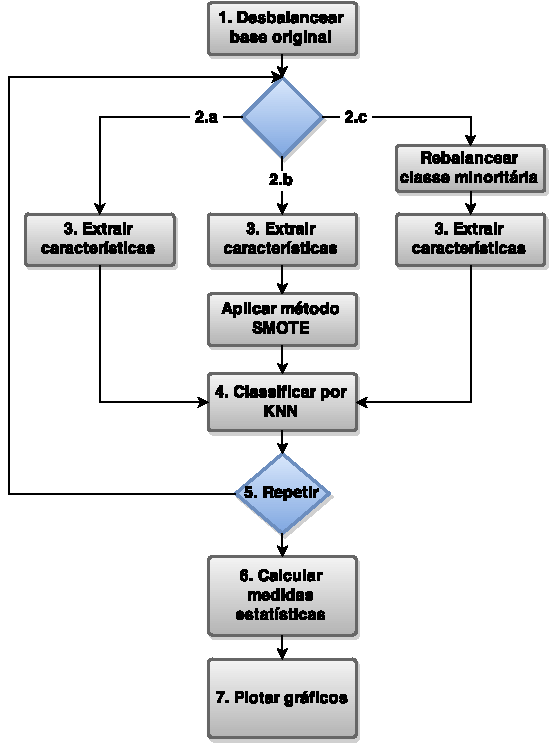
\includegraphics[scale=1.1]{\detokenize{figuras/flow_main.pdf}}
\caption[Fluxo de operações para obtenção dos resultados do rebalanceamento de classes]{Fluxo de operações para obtenção dos resultados do rebalanceamento de classes. \textit{Fonte:~Elaborado pela autora.}}
\label{fig:fluxo}
\end{figure}

Procurando estabilidade dos resultados obtidos com a geração das imagens artificiais, foi identificada a necessidade de controlar a remoção de imagens da base no momento da criação da base desbalanceada. Assim, os resultados foram obtidos a partir de uma forma de validação K-fold com o objetivo de prover mais robustez ao sistema. A Figura \ref{fig:folds} ilustra como tal validação foi realizada, utilizando como exemplo uma base com duas classes de imagens. Primeiramente as imagens foram divididas de forma aleatória em $k=5$ folds em cada classe. Depois, as duas classes compõem 40 configurações, consistindo em: um fold para teste e os outros para treino na classe que permanecerá balanceada; e um de teste e um de treino para a classe que os métodos de processamento irão rebalancear. E isso é repetido para todas as classes. Se originalmente a base é naturalmente desbalanceada, então um fold será utilizado para teste e os restantes para treino para todas as classes.

\begin{figure}[!htbp]
\centering
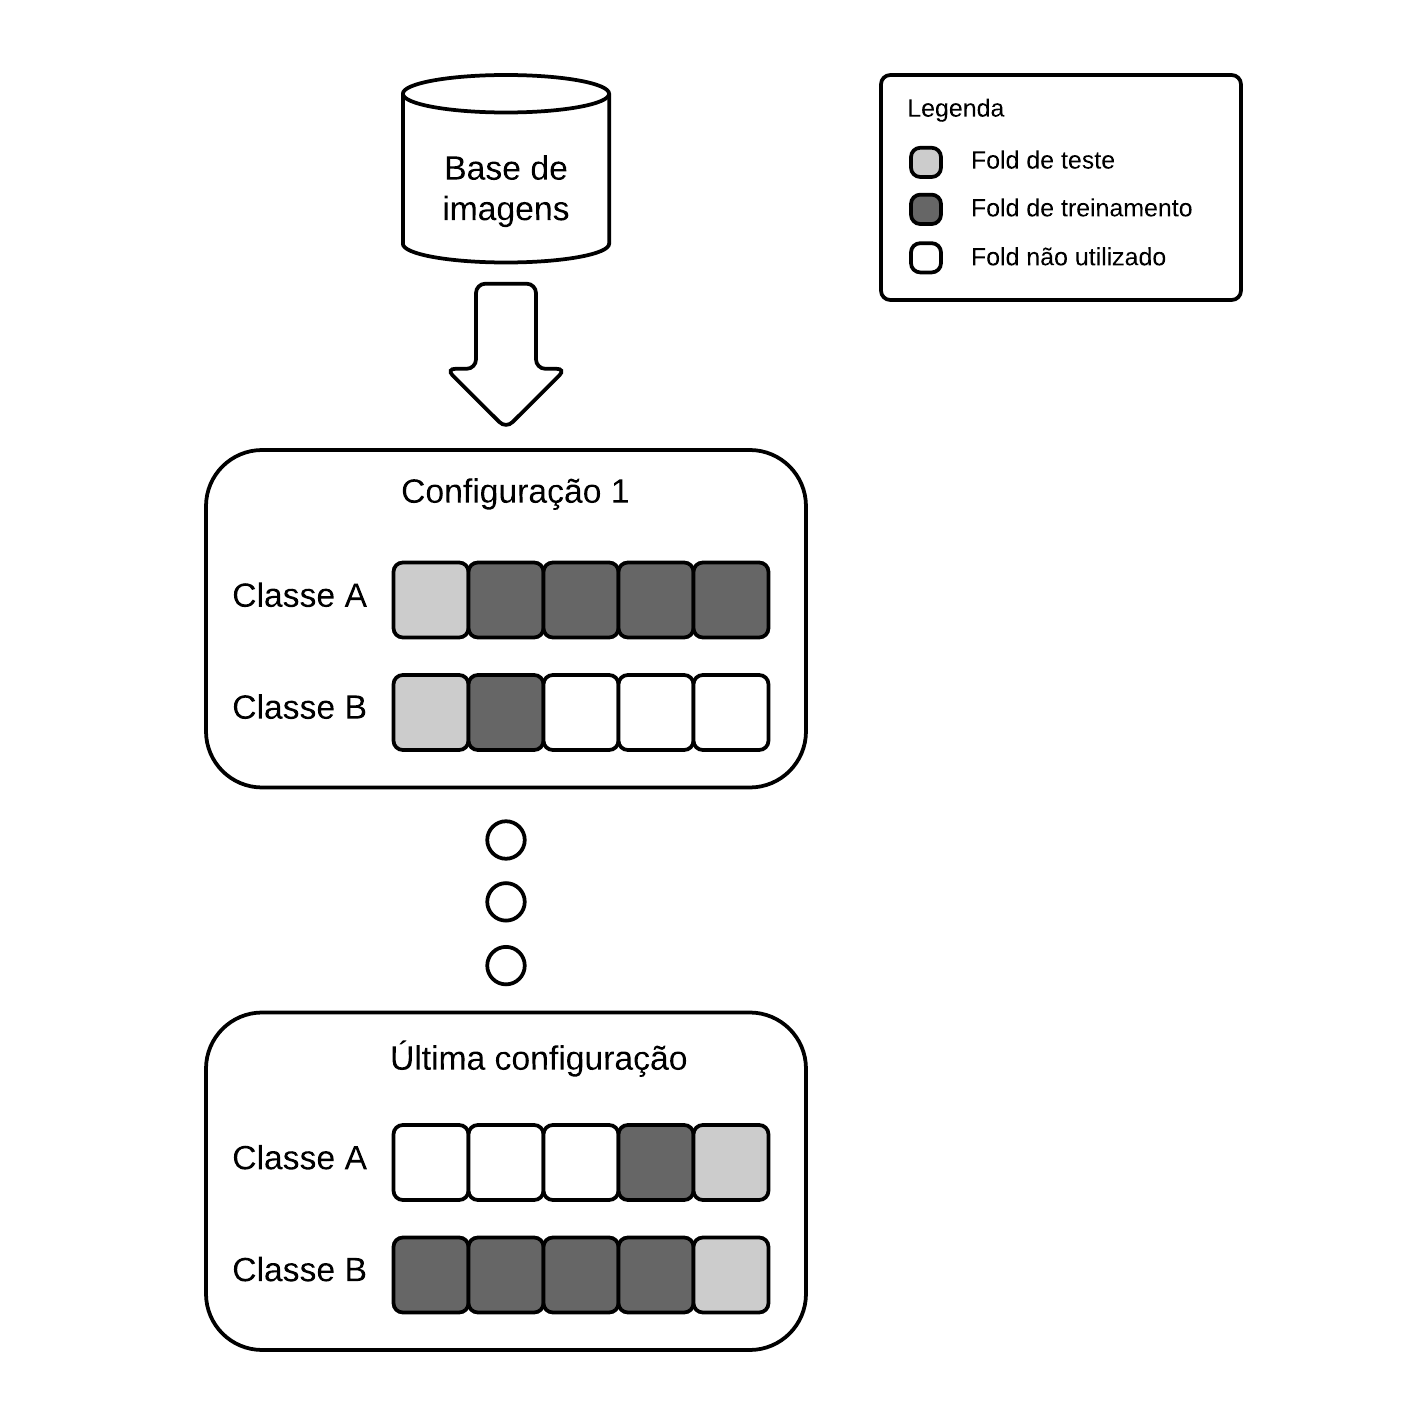
\includegraphics[scale=0.3]{\detokenize{figuras/folds_chart.png}}
\caption[]{\textit{Fonte:~Elaborado pela autora.}}
\label{fig:folds}
\end{figure}

A seguir, para cada experimento realizado são descritos: a base de imagens utilizada; o protocolo e parâmetros adotados; e por fim os resultados obtidos a partir de seu uso são mostrados e discutidos.

%%%%%%%%%%%%%%%%%%%%%%%%%%%%%%%%%%%%%%%%%%%%%%%%%%%%%%%%%%%%%%%%%%%%%%%%%%%%%%%%
\FloatBarrier
\subsection{Experimento 1: duas classes bem discriminadas}

Neste experimento foram utilizadas duas classes com cores bem distintas entre elas. Por tal razão, um sub-experimento de visualização foi realizado para análise do espaço de características. Como o foco é na visualização do espaço de características, é relevante ter o modelo do espaço ideal das classes balanceadas, por isso esse experimento em específico não trata de uma base naturalmente desbalanceada.

%-------------------------------------------------------------------------------
\begin{itemize}

\item[] \textbf{Protocolo}

\begin{enumerate}
\item \textbf{Imagens originais}: Duas classes da base Corel-1000: \emph{Cavalos} e \emph{Elefantes}. As classes estão exemplificadas na Figura \ref{fig:exp1:base}. A principal característica dessas imagens é a diferença das cores das imagens. Apesar de haverem casos de confusão, são classes que podem ser consideradas bem discriminadas.

\begin{minipage}{\linewidth}
  \begin{figure}[H]
    \subfloat{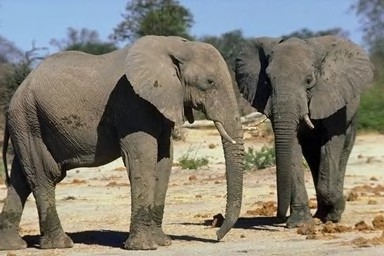
\includegraphics[width=0.45\linewidth]{\detokenize{figuras/corel_original4.jpg}}}
    \subfloat{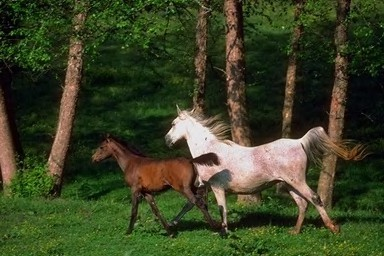
\includegraphics[width=0.45\linewidth]{\detokenize{figuras/cavalo-original2.png}}}

    \caption[Classes cavalo e elefante utilizadas neste experimento. São duas classes bem discriminadas com 100 imagens cada, originalmente da base de imagens Corel.]{Classes cavalo e elefante utilizadas neste experimento. São duas classes bem discriminadas com 100 imagens cada, originalmente da base de imagens Corel. \textit{Fonte:~Elaborado pela autora.}}
    \label{fig:exp1:base}
  \end{figure}
\end{minipage}

\item \textbf{Desbalanceamento}: para o sub-experimento de visualização, cada classe foi dividida em 50\% para treino e 50\% para teste. Após, a classe \emph{Cavalos} sofreu remoção de 50\% do seu conjunto de treino. Já para a análise estatística do experimento, todas as 40 configurações de folds com $k=5$ foram realizadas (padronização anteriormente descrita na Figura~\ref{fig:folds});
\item \textbf{Método para geração artificial}: para a visualização do espaço de características foi utilizado o método de mistura de duas imagens originais, exemplificado na Figura~\ref{fig:mistura}. Para a análise do boxplot de \textit{f1-scores}, todas as gerações foram testadas;

\begin{minipage}{\linewidth}
  \begin{figure}[H]
    \subfloat[Original]{
      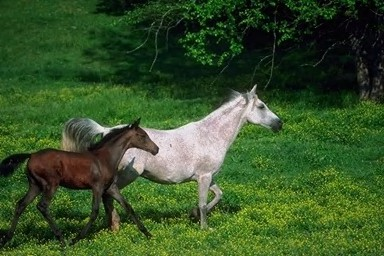
\includegraphics[width=.33\linewidth]{\detokenize{figuras/cavalo-original.png}}
    }
    \subfloat[Original]{
      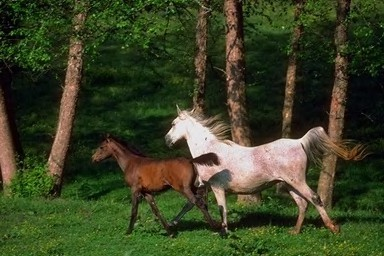
\includegraphics[width=.33\linewidth]{\detokenize{figuras/cavalo-original2.png}}
    }
    \subfloat[Mistura]{
      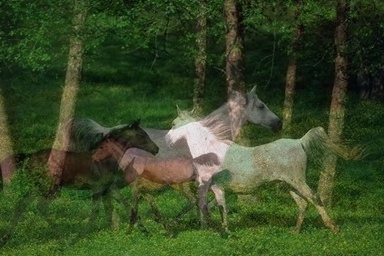
\includegraphics[width=.33\linewidth]{\detokenize{figuras/cavalo-blend.png}}
    }
    \caption[Exemplo da geração artificial de imagens com o método de mistura para as classes \emph{Elefante} e \emph{Cavalo} da Corel-1000.]{Exemplo da geração artificial de imagens com o método de mistura para as classes \emph{Elefante} e \emph{Cavalo} da Corel-1000. \textit{Fonte:~Elaborado pela autora.}}
    \label{fig:mistura}
  \end{figure}
\end{minipage}

\item \textbf{Conversão em escala de cinza}: método \emph{Intensidade};
\item \textbf{Extração de características}: classificação de pixels de borda e interior (BIC);
\item \textbf{Classificação}: classificador supervisionado KNN com $K=1$ (para mais detalhes ver Seção~\ref{sec:knn});
\item \textbf{Projeção multidimensional}: projetados os dois componentes principais encontrados ao aplicar PCA nos vetores de características para redução de dimensionalidade (Seção~\ref{sec:pca}).
\end{enumerate}

%-------------------------------------------------------------------------------
\FloatBarrier
\item[] \textbf{Visualização}

As classes \emph{Elefantes} e \emph{Cavalos} possuem 100 imagens cada. O primeiro passo foi remover imagens de uma das classes, tornando a base desbalanceada. Na Figura~\ref{fig:desbalanceado} está ilustrada a remoção de 50\% das imagens de treino da classe \emph{Cavalos}, originalmente balanceada. Essa e as próximas projeções desta seção foram obtidas com a técnica para redução de dimensionalidade PCA, descrita na Seção~\ref{sec:pca}, e são referentes aos dois componentes principais com maiores autovalores.

\begin{minipage}{\linewidth}
  \begin{figure}[H]
    \subfloat[Original]{
      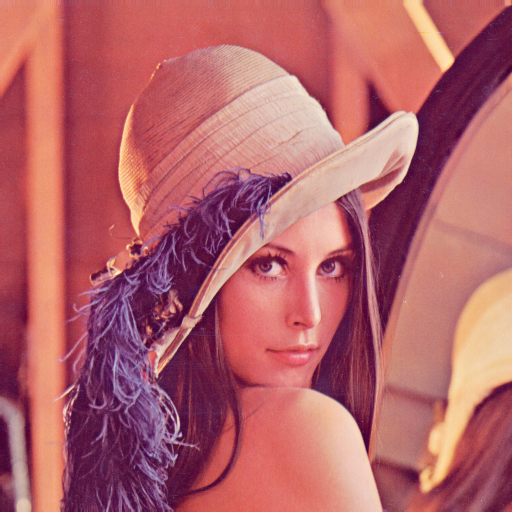
\includegraphics[width=.49\linewidth]{\detokenize{figuras/visualizacao/original.png}}
    }
    \subfloat[Desbalanceado]{
      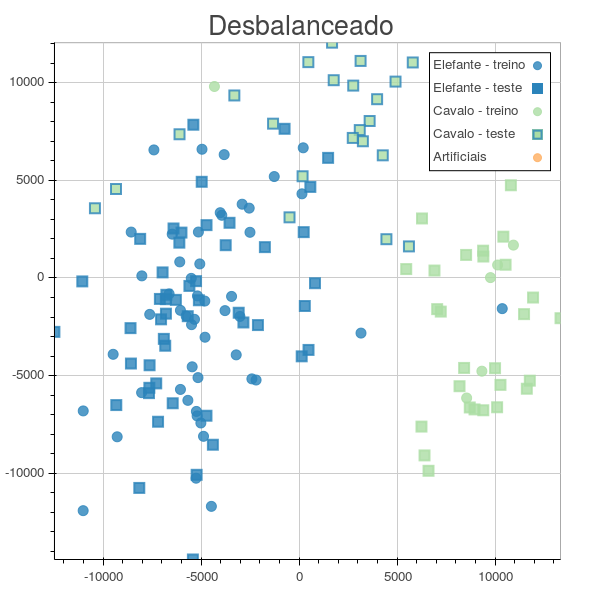
\includegraphics[width=.49\linewidth]{\detokenize{figuras/visualizacao/desbalanceado-fixed.png}}
    }
    \caption[À esquerda a projeção dos dois componentes principais obtidos com a aplicação de PCA nas classes \emph{Elefante} -- em azul -- e \emph{Cavalo} -- em verde. À direita, as mesmas classes após a remoção de 50\% das imagens de treino da classe \emph{cavalo}. A diferença dos marcadores consiste na definição de imagens para treino e teste não existente nas classes originais.]{À esquerda a projeção dos dois componentes principais obtidos com a aplicação de PCA nas classes \emph{Elefante} -- em azul -- e \emph{Cavalo} -- em verde. À direita, as mesmas classes após a remoção de 50\% das imagens de treino da classe \emph{cavalo}. A diferença dos marcadores consiste na definição de imagens para treino e teste não existente nas classes originais. \textit{Fonte:~Elaborado pela autora.}}
    \label{fig:desbalanceado}
  \end{figure}
\end{minipage}

Os resultados da classificação dos três experimentos utilizando KNN reportou que o \textit{f1-score} da geração artificial de imagens utilizando o método de mistura teve um ganho satisfatório em relação ao rebalanceamento no espaço de características com o SMOTE (apresentado na Figura \ref{fig:resultados:1:vis}). Foi utilizado BIC como método de extração de características e Intensidade como método de conversão em escala de cinza. Para essa combinação, a geração de imagens utilizando mistura se mostrou favorável e portanto a visualização do espaço de características apresenta esse método como geração.

\begin{minipage}{\linewidth}
  \begin{figure}[H]
      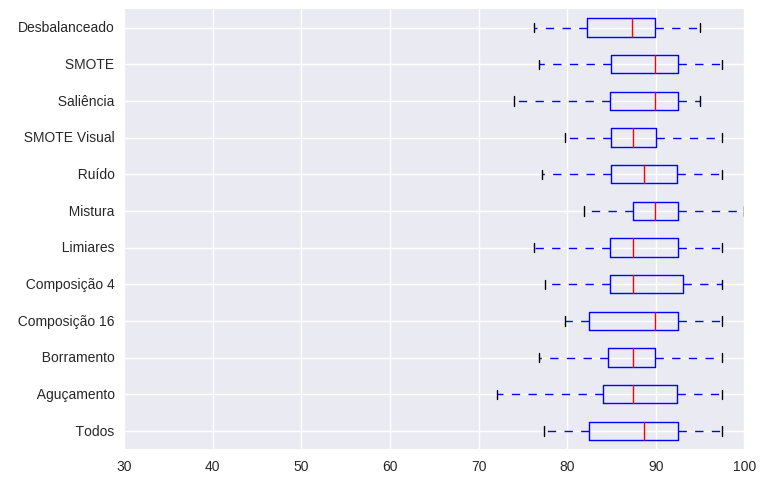
\includegraphics[width=\linewidth]{\detokenize{figuras/resultados/1/BIC_Intensity_elefante-cavalo.png}}
    \caption[Resultados de \textit{f1-score} para as classes \emph{Cavalo} e \emph{Elefante} da base Corel. Foi utilizado BIC como método de extração de características e Intensidade como método de conversão em escala de cinza. Para essa combinação, a geração de imagens utilizando mistura se mostrou favorável.]{Resultados de \textit{f1-score} para as classes \emph{Cavalo} e \emph{Elefante} da base Corel. Foi utilizado BIC como método de extração de características e Intensidade como método de conversão em escala de cinza. Para essa combinação, a geração de imagens utilizando mistura se mostrou favorável. \textit{Fonte:~Elaborado pela autora.}}
    \label{fig:resultados:1:vis}
  \end{figure}
\end{minipage}

\begin{table}[!htbp]
\centering
\caption{}
\label{fig:resultados:1:tabvis}
\begin{tabular}{|l|c|c|}
\hline
\textbf{Intensidade e BIC} & \textbf{Média} & \textbf{Desvio padrão} \\ \hline
Todos                      & 88.07          & 5.30                   \\ \hline
Aguçamento                 & 86.65          & 7.00                   \\ \hline
Borramento                 & 87.17          & 5.10                   \\ \hline
Composição 16              & 88.16          & 5.32                   \\ \hline
Composição 4               & 88.12          & 5.45                   \\ \hline
Limiares                   & 87.65          & 5.10                   \\ \hline
Mistura                    & \textbf{88.84} & 5.03          \\ \hline
Ruído                      & 87.95          & 5.75                   \\ \hline
SMOTE Visual               & 87.69          & 5.28                   \\ \hline
Saliência                  & 88.09          & 5.58                   \\ \hline
SMOTE                      & 88.55          & 5.21                   \\ \hline
Desbalanceado              & 85.82          & 5.69                   \\ \hline
\end{tabular}
\end{table}

Para confirmar se a geração de imagens inseriu mais informação na classe minoritária do que apenas povoar os espaços entre os exemplos (i.e.\ SMOTE), a classe rebalanceada utilizando ambos métodos está demonstrada na Figura~\ref{fig:compara_vis_treino_fixed}. Em laranja estão representados os novos exemplos de treinamento, projetados no plano da base original balanceada.

\begin{minipage}{\linewidth}
  \begin{figure}[H]
    \subfloat[Smote]{      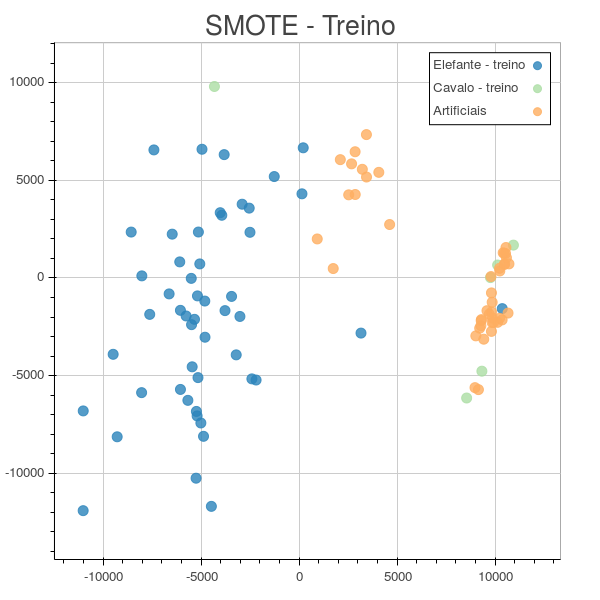
\includegraphics[width=.5\linewidth]{\detokenize{figuras/visualizacao/smote-treino-fixed.png}}
    }
    \subfloat[Geração artificial]{      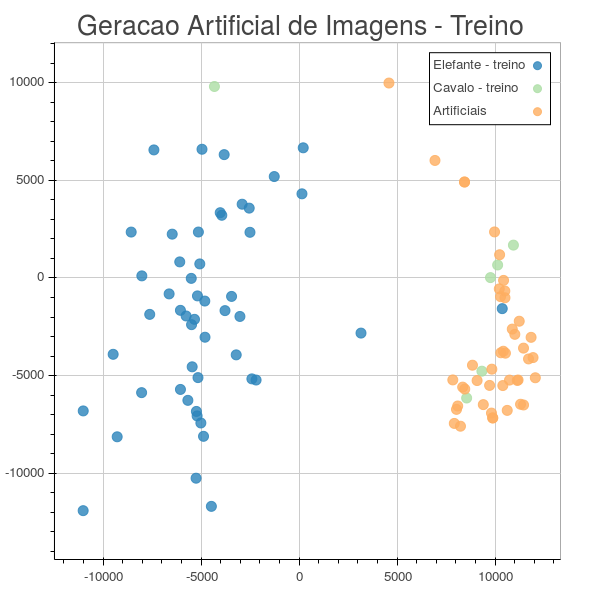
\includegraphics[width=.5\linewidth]{\detokenize{figuras/visualizacao/geracao-treino-fixed.png}}
    }
  \caption[Comparação dos exemplos de treinamento da geração com SMOTE e no campo visual. Em laranja estão representados os novos exemplos, projetados no plano da base original balanceada.]{Comparação dos exemplos de treinamento da geração com SMOTE e no campo visual. Em laranja estão representados os novos exemplos, projetados no plano da base original balanceada. \textit{Fonte:~Elaborado pela autora.}}
  \label{fig:compara_vis_treino_fixed}
  \end{figure}
\end{minipage}

Após o treinamento realizado com as novas imagens geradas e as originais, o conjunto de teste foi fornecido ao classificador 1-NN e o resultado das predições está ilustrado na Figura~\ref{fig:compara_vis_teste}. A cor no interior dos marcadores quadrados representa a classe real dos exemplos e a borda representa a classe predita pelo classificador. Nota-se que a melhoria na classificação com a geração de imagens fica visível e corresponde ao aumento do \textit{f1-score}.


\begin{minipage}{\linewidth}
  \begin{figure}[H]
    \subfloat[Smote]{
      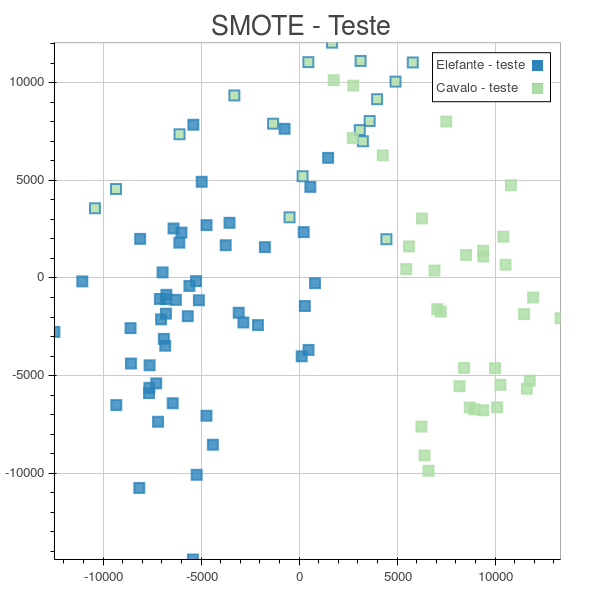
\includegraphics[width=.5\linewidth]{\detokenize{figuras/visualizacao/smote-teste-fixed.png}}
    }
    \subfloat[Geração artificial]{
      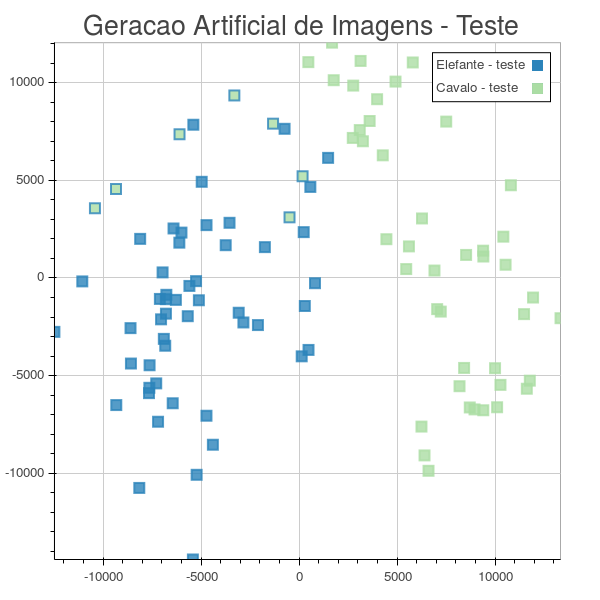
\includegraphics[width=.5\linewidth]{\detokenize{figuras/visualizacao/geracao-teste-fixed.png}}
    }
  \caption[Resultado do teste da classificação com 1-NN após o treinamento realizado com as bases rebalanceadas. A cor no interior dos marcadores quadrados representa a classe real dos exemplos e a borda representa a classe predita pelo classificador.]{Resultado do teste da classificação com 1-NN após o treinamento realizado com as bases rebalanceadas. A cor no interior dos marcadores quadrados representa a classe real dos exemplos e a borda representa a classe predita pelo classificador. \textit{Fonte:~Elaborado pela autora.}}
  \label{fig:compara_vis_teste}
\end{figure}
\end{minipage}

De uma forma geral, pode-se dizer que a geração de imagens melhorou a definição da classe minoritária e foi o método que mais se assemelhou à distribuição dos dados originais. Além disso, um dos problemas do SMOTE pode ser verificado nessas projeções: ao realizar a interpolação dos vetores de características originais, exemplos podem ser criados em regiões do espaço que fazem parte da outra classe. Ficou claro também que o método SMOTE não possui capacidade de extrapolar a sua região, como pode ser observado no grupo de exemplos gerados à direita do espaço de características. O SMOTE gerou novos elementos próximos a uma linha reta, enquanto a geração de imagens proporcionou uma abrangência maior em volta desse espaço, com maior dispersão.

Na Figura \ref{fig:region} é possível visualizar a região de decisão, observando suas modificações frente aos métodos. Pode ser observado que em ambas técnicas a região da classe minoritária apresenta-se melhor representada. Além disso, é possível verificar que o SMOTE ocasionou uma certa ``invasão'' do espaço de características da classe majoritária.

\begin{minipage}{\linewidth}
  \begin{figure}[H]
    \subfloat[Smote]{
      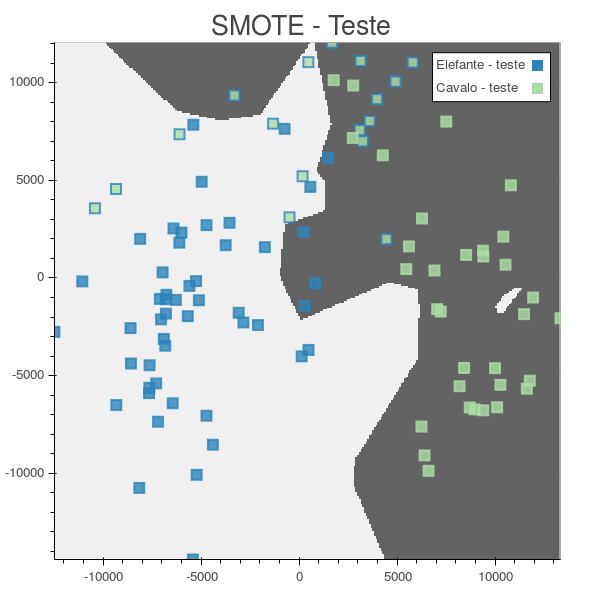
\includegraphics[width=.33\linewidth]{\detokenize{figuras/visualizacao/smote-teste-region.png}}
    }
    \subfloat[Geração artificial]{
      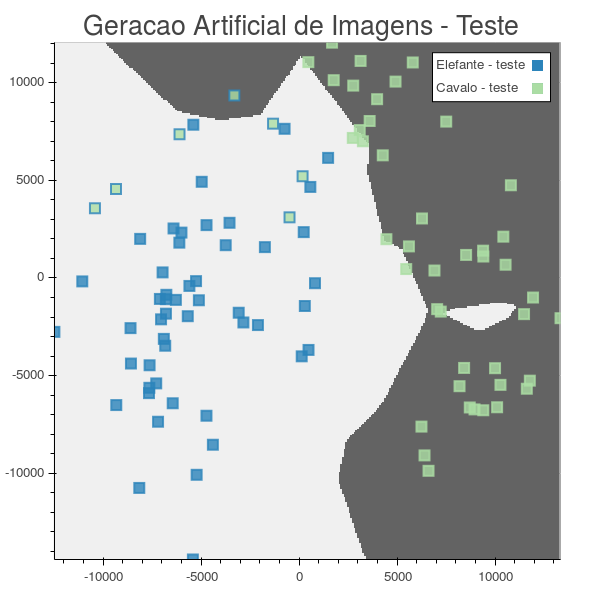
\includegraphics[width=.33\linewidth]{\detokenize{figuras/visualizacao/geracao-teste-region.png}}
    }
    \subfloat[Desbalanceado]{
      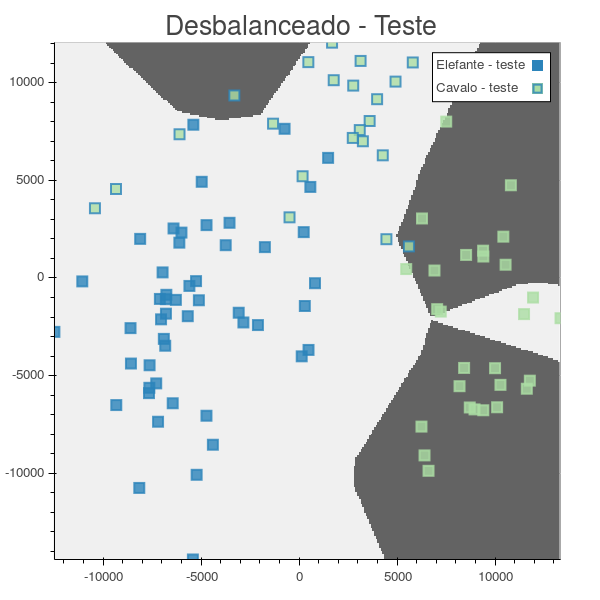
\includegraphics[width=.33\linewidth]{\detokenize{figuras/visualizacao/desbalanceado-teste-region.png}}
    }
  \caption[Região de decisão com K-NN (K = 1). Pode ser observado que em ambas técnicas a região da classe minoritária apresenta-se melhor representada. Além disso, é possível verificar que o SMOTE ocasionou uma certa ``invasão'' do espaço de características da classe majoritária.]{Região de decisão com K-NN (K = 1). Pode ser observado que em ambas técnicas a região da classe minoritária apresenta-se melhor representada. Além disso, é possível verificar que o SMOTE ocasionou uma certa ``invasão'' do espaço de características da classe majoritária. \textit{Fonte:~Elaborado pela autora.}}
  \label{fig:region}
  \end{figure}
\end{minipage}

Em todas as figuras anteriores relacionadas a essa visualização, os exemplos foram projetados no plano criado pelas suas componentes principais com maior autovalores da base original balanceada. Se após a geração de novos exemplos essas componentes forem recalculadas (Figura \ref{fig:compara_vis_treino}), pode-se notar que a geração de imagens artificiais proporciona a criação de um subespaço que melhor discretiza as classes, quando comparado com SMOTE ou com a base desbalanceada.

\begin{minipage}{\linewidth}
  \begin{figure}[H]
    \subfloat[Smote]{
      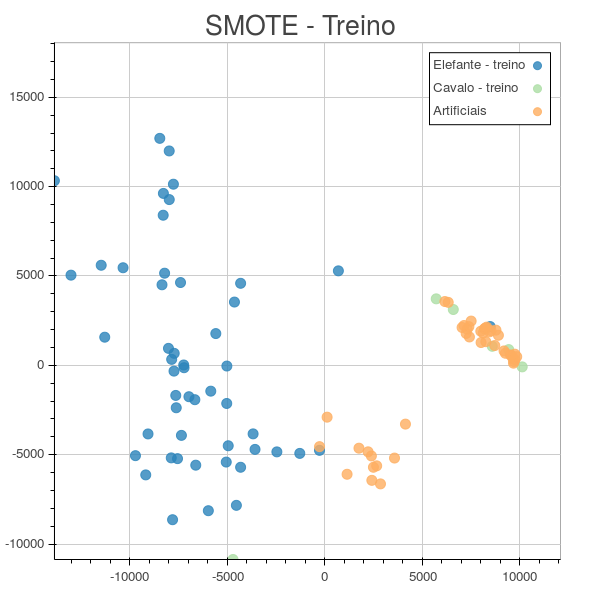
\includegraphics[width=.33\linewidth]{\detokenize{figuras/visualizacao/smote-treino.png}}
    }
    \subfloat[Geração artificial]{
      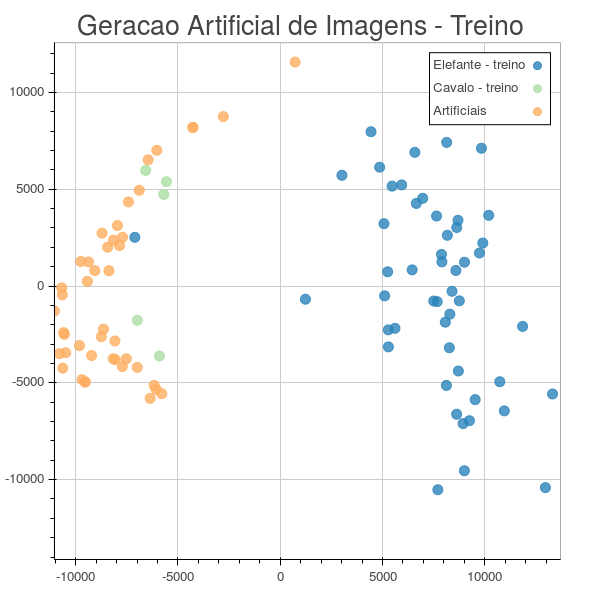
\includegraphics[width=.33\linewidth]{\detokenize{figuras/visualizacao/geracao-treino.png}}
    }
    \subfloat[Desbalanceado]{
      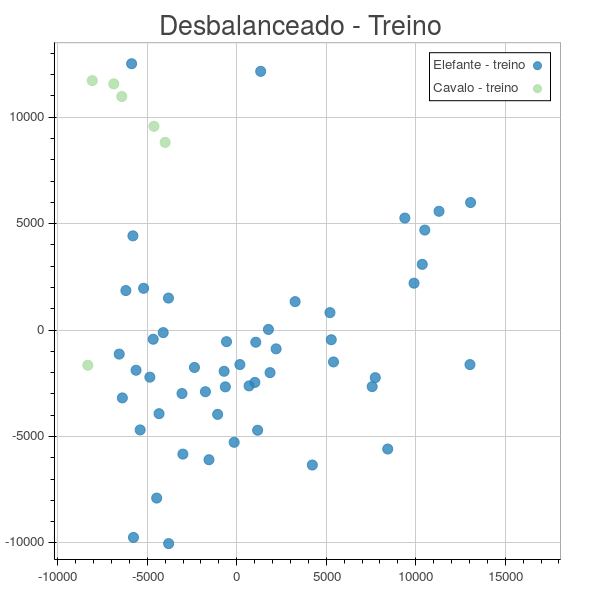
\includegraphics[width=.33\linewidth]{\detokenize{figuras/visualizacao/desbalanceado-treino.png}}
    }
  \caption[Melhores subespaços encontrados após a geração de novos exemplos para o SMOTE e para a geração artificial de imagens, e após a remoção de imagens para a projeção dos dados desbalanceados. Pode-se notar que a geração de imagens artificiais proporciona a criação de um subespaço que melhor discretiza as classes, quando comparado com SMOTE ou com a base desbalanceada.]{Melhores subespaços encontrados após a geração de novos exemplos para o SMOTE e para a geração artificial de imagens, e após a remoção de imagens para a projeção dos dados desbalanceados. Pode-se notar que a geração de imagens artificiais proporciona a criação de um subespaço que melhor discretiza as classes, quando comparado com SMOTE ou com a base desbalanceada. \textit{Fonte:~Elaborado pela autora.}}
  \label{fig:compara_vis_treino}
  \end{figure}
\end{minipage}

Como relatado no início desse experimento, o extrator de características utilizado foi o BIC. Fundamentalmente ele captura informações de intensidade de cor das imagens. Na Figura~\ref{fig:vis_images} as próprias imagens foram utilizadas como marcadores na projeção do melhor subespaço após a geração artificial com o método de mistura. É nítido o impacto da etapa de extração de características na separação das classes e também no método de geração de imagens antes dessa extração.

\begin{minipage}{\linewidth}
  \begin{figure}[H]
    \begin{center}
      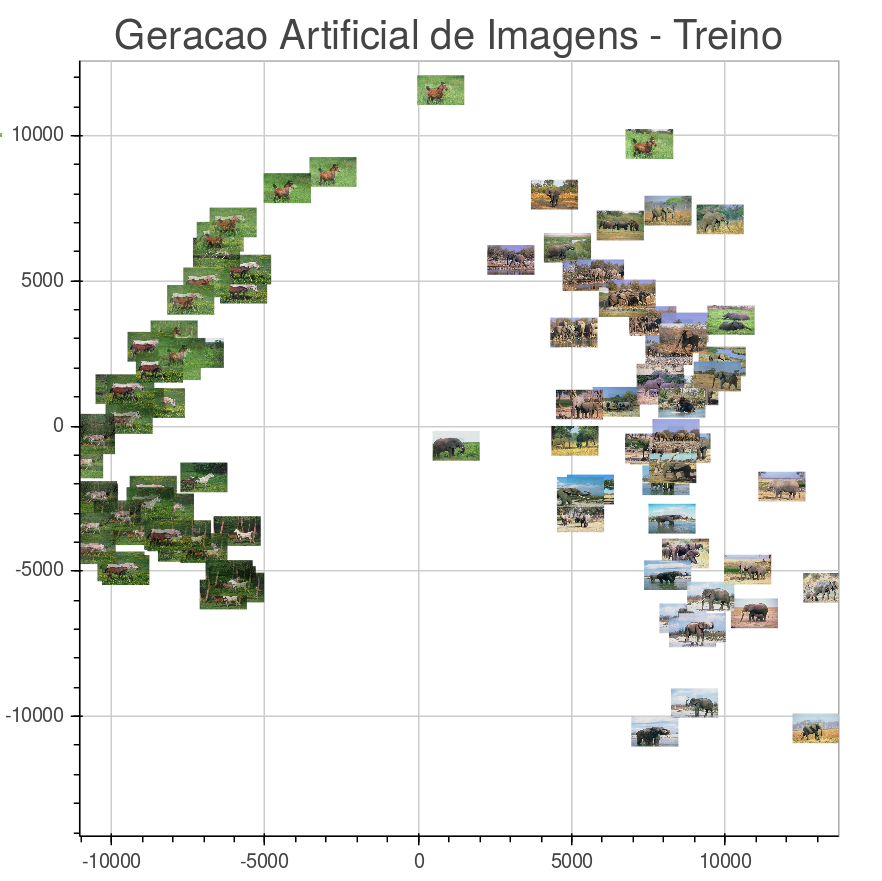
\includegraphics[width=.6\linewidth]{\detokenize{figuras/visualizacao/vis-images.png}}
    \end{center}
  \caption[Visualização do impacto do método de extração de características na separação entre classes. Possível verificar que o BIC utiliza as intensidades como principal representação de uma imagem.]{Visualização do impacto do método de extração de características na separação entre classes. Possível verificar que o BIC utiliza as intensidades como principal representação de uma imagem. \textit{Fonte:~Elaborado pela autora.}}
  \label{fig:vis_images}
\end{figure}
\end{minipage}

%-------------------------------------------------------------------------------
\item[] \textbf{Resultado da melhor combinação dos métodos de extração e conversão para escala de cinza}

\begin{minipage}{\linewidth}
  \begin{figure}[H]
  \begin{center}
      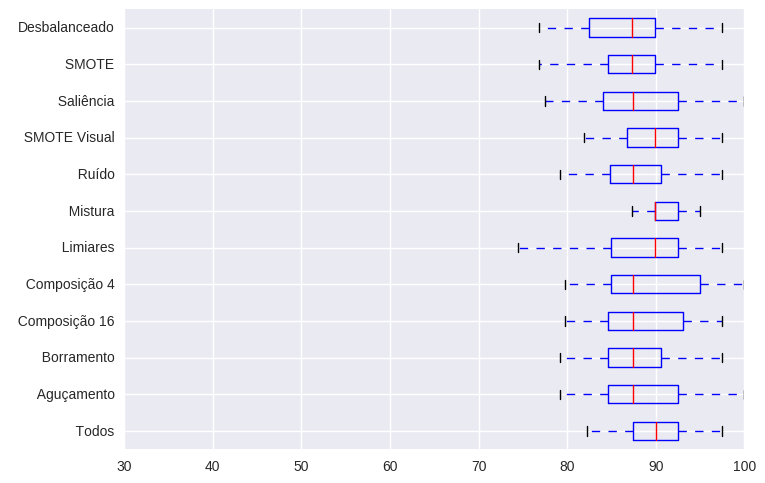
\includegraphics[width=\linewidth]{\detokenize{figuras/resultados/1/GCH_Gleam_elefante-cavalo.png}}
  \end{center}
  \caption[]{Conversão em escala de cinza com Gleam e GCH como método de extração de características. \textit{Fonte:~Elaborado pela autora.}}
  \label{fig:resultados:1:melhor}
\end{figure}
\end{minipage}

\begin{table}[!htbp]
\centering
\caption{}
\label{fig:resultados:1:tabmelhor}
\begin{tabular}{|l|c|c|}
\hline
\textbf{Gleam e GCH} & \textbf{Média} & \textbf{Desvio padrão} \\ \hline
Todos                & 90.32          & 4.14                   \\ \hline
Aguçamento           & 88.09          & 5.78                   \\ \hline
Borramento           & 87.97          & 4.86                   \\ \hline
Composição 16        & 89.14          & 5.24                   \\ \hline
Composição 4         & 89.24          & 5.42                   \\ \hline
Limiares             & 88.78          & 5.51                   \\ \hline
Mistura              & \textbf{90.64} & 3.08          \\ \hline
Ruído                & 88.31          & 4.96                   \\ \hline
SMOTE Visual         & 89.62          & 4.06                   \\ \hline
Saliência            & 88.01          & 5.59                   \\ \hline
SMOTE                & 87.71          & 5.47                   \\ \hline
Desbalanceado        & 87.09          & 5.31                   \\ \hline
\end{tabular}
\end{table}

\begin{minipage}{\linewidth}
  \begin{figure}[H]
    \subfloat[Original]{
      \includegraphics[width=.33\linewidth]{\detokenize{figuras/resultados/1/original-mistura.png}}
    }
    \subfloat[Original]{
      \includegraphics[width=.33\linewidth]{\detokenize{figuras/resultados/1/original2-mistura.png}}
      }
    \subfloat[Mistura]{
      \includegraphics[width=.33\linewidth]{\detokenize{figuras/resultados/1/resultado-mistura.png}}
    }
   \caption[]{ \textit{Fonte:~Elaborado pela autora.}}
   \label{fig:resultados:1:mistura}
  \end{figure}
\end{minipage}

%-------------------------------------------------------------------------------
\item[] \textbf{Resultado da maior variância obtida com a combinação dos métodos de extração e conversão para escala de cinza}

\begin{minipage}{\linewidth}
  \begin{figure}[H]
    \begin{center}
      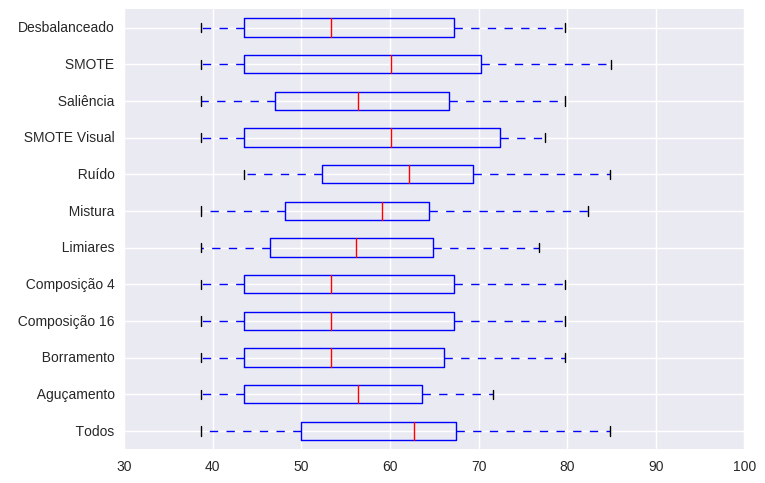
\includegraphics[width=\linewidth]{\detokenize{figuras/resultados/1/HOG_MSB_elefante-cavalo.png}}
    \end{center}
    \caption[]{Conversão em escala de cinza com MSB e HOG como método de extração de características. \textit{Fonte:~Elaborado pela autora.}}
    \label{fig:resultados:1:pior}
  \end{figure}
\end{minipage}

\begin{table}[!htbp]
\centering
\caption{}
\label{fig:resultados:1:tabpior}
\begin{tabular}{|l|c|c|}
\hline
\textbf{MSB e HOG} & \textbf{Média}     & \textbf{Desvio padrão} \\ \hline
Todos              & 59.870730          & 12.129320              \\ \hline
Aguçamento         & 54.343938          & 10.167572              \\ \hline
Borramento         & 55.588173          & 13.275734              \\ \hline
Composição 16      & 55.667145          & 13.341421              \\ \hline
Composição 4       & 55.392485          & 13.212076              \\ \hline
Limiares           & 55.023675          & 10.854750              \\ \hline
Mistura            & 59.539932          & 10.952548              \\ \hline
Ruído              & \textbf{62.580685} & 11.088673              \\ \hline
SMOTE Visual       & 58.318472          & 14.690079              \\ \hline
Saliência          & 56.269225          & 12.329254              \\ \hline
SMOTE              & 59.163262          & 14.082027              \\ \hline
Desbalanceado      & 55.667145          & 13.341421              \\ \hline
\end{tabular}
\end{table}

\begin{minipage}{\linewidth}
  \begin{figure}[H]
    \subfloat[Original]{
      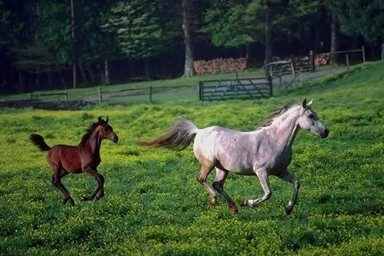
\includegraphics[width=.5\linewidth]{\detokenize{figuras/resultados/1/original-ruido.png}}
    }
    \subfloat[Ruído]{
      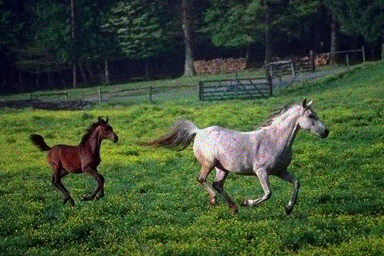
\includegraphics[width=.5\linewidth]{\detokenize{figuras/resultados/1/resultado-ruido.png}}
    }
 \caption[]{ \textit{Fonte:~Elaborado pela autora.}}
 \label{fig:resultados:1:ruido}
\end{figure}
\end{minipage}

%-------------------------------------------------------------------------------
\item[] \textbf{Discussão}

\end{itemize}


%%%%%%%%%%%%%%%%%%%%%%%%%%%%%%%%%%%%%%%%%%%%%%%%%%%%%%%%%%%%%%%%%%%%%%%%%%%%%%%%
\FloatBarrier
\subsection{Experimento 2: duas classes bem sobrepostas}

\begin{itemize}
%-------------------------------------------------------------------------------
\item[] \textbf{Base de Imagens}

% \begin{figure}[!htbp]
%   \begin{center}
%     \begin{subfigure}{.49\linewidth}
%       \centering
%       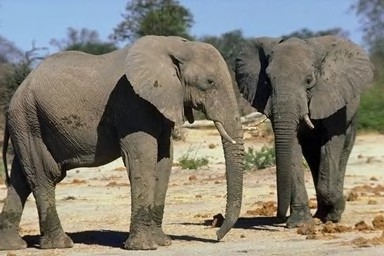
\includegraphics[width=\linewidth]{\detokenize{figuras/corel_original4.jpg}}
%     \end{subfigure}
%     \begin{subfigure}{.49\linewidth}
%       \centering
%       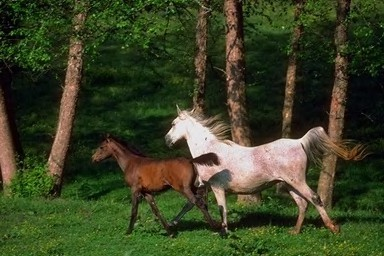
\includegraphics[width=\linewidth]{\detokenize{figuras/cavalo-original2.png}}
%     \end{subfigure}
%   \end{center}
%   \caption{Remoção de 50\% das imagens de treino da classe Cavalo.}
%   \label{fig:exp1:base}
% \end{figure}

%-------------------------------------------------------------------------------
\item[] \textbf{Protocolo}

O seguinte protocolo foi seguido para a obtenção dos resultados:

\begin{enumerate}
\item \textbf{Classes de imagens originais}:
\item \textbf{Desbalanceamento}:
\item \textbf{Método para geração artificial}:
\item \textbf{Quantização}:
\item \textbf{Extração de características}:
\item \textbf{Classificação}:
\end{enumerate}

%-------------------------------------------------------------------------------
\item[] \textbf{Resultado da melhor combinação dos métodos de extração e conversão para escala de cinza}

\begin{figure}[!htbp]
  \begin{center}
      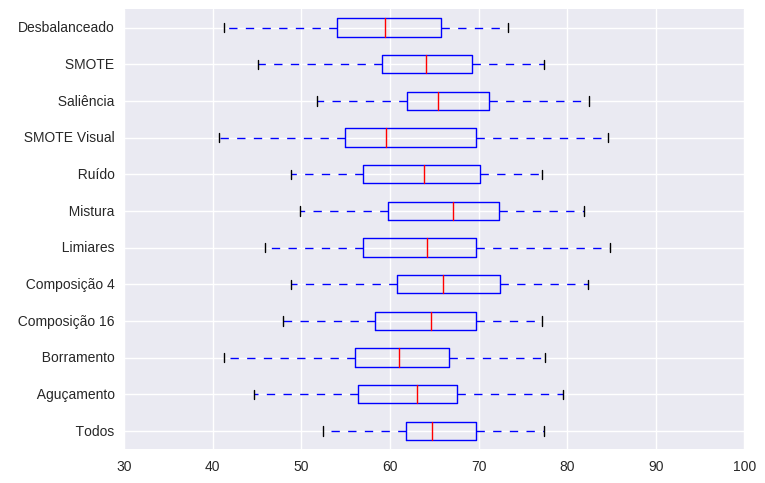
\includegraphics[width=\linewidth]{\detokenize{figuras/resultados/2/BIC_Luminance_praia-montanha.png}}
  \end{center}
  \caption[]{Conversão em escala de cinza com Luminância e BIC como método de extração de características. \textit{Fonte:~Elaborado pela autora.}}
  \label{fig:resultados:2:pior}
\end{figure}


\begin{table}[!htbp]
\centering
\caption{}
\label{my-label}
\begin{tabular}{|l|c|c|}
\hline
\textbf{BIC Luminance} & \textbf{Média} & \textbf{Desvio padrão} \\ \hline
Todos                  & 65.21          & 7.54                   \\ \hline
Aguçamento             & 62.30          & 7.85                   \\ \hline
Borramento             & 61.24          & 7.55                   \\ \hline
Composição 16          & 64.23          & 7.31                   \\ \hline
Composição 4           & 65.65          & 8.27                   \\ \hline
Limiares               & 63.69          & 8.77                   \\ \hline
Mistura                & 65.41          & 8.20                   \\ \hline
Ruído                  & 63.50          & 8.05                   \\ \hline
SMOTE Visual           & 61.55          & 9.44                   \\ \hline
Saliência              & \textbf{65.69} & 6.63                   \\ \hline
SMOTE                  & 63.58          & 7.74                   \\ \hline
Desbalanceado          & 59.49          & 8.11                   \\ \hline
\end{tabular}
\end{table}

\begin{minipage}{\linewidth}
  \begin{figure}[H]
    \subfloat[Original]{  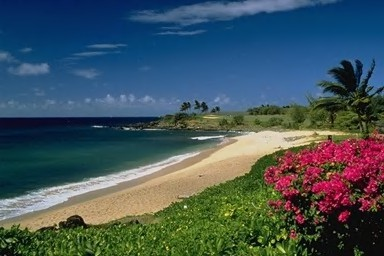
\includegraphics[width=.33\linewidth]{\detokenize{figuras/resultados/2/original-saliencia.png}}
    }
    \subfloat[Original]{
      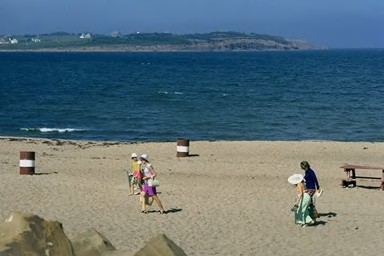
\includegraphics[width=.33\linewidth]{\detokenize{figuras/resultados/2/original2-saliencia.png}}
    }
    \subfloat[Saliência]{
      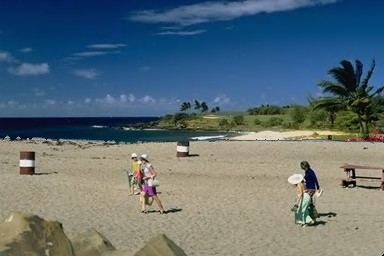
\includegraphics[width=.33\linewidth]{\detokenize{figuras/resultados/2/resultado-saliencia.png}}
    }
 \caption[]{\textit{Fonte:~Elaborado pela autora.}}
 \label{fig:resultados:2:saliencia}
\end{figure}
\end{minipage}

%-------------------------------------------------------------------------------
\item[] \textbf{Resultado da maior variância obtida com a combinação dos métodos de extração e conversão para escala de cinza}

\begin{minipage}{\linewidth}
  \begin{figure}[H]
  \begin{center}
      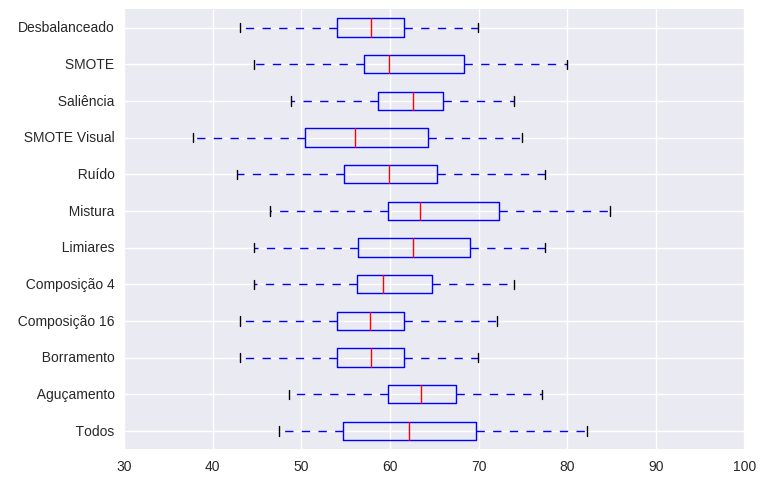
\includegraphics[width=\linewidth]{\detokenize{figuras/resultados/2/HOG_Intensity_praia-montanha.png}}
  \end{center}
  \caption[]{Conversão em escala de cinza com Intensidade e HOG como método de extração de características. \textit{Fonte:~Elaborado pela autora.}}
  \label{fig:resultados:2:pior}
\end{figure}
\end{minipage}

\begin{table}[!htbp]
\centering
\caption{}
\label{my-label}
\begin{tabular}{|l|c|c|}
\hline
\textbf{Intensidade e HOG} & \textbf{Média}     & \textbf{Desvio padrão} \\ \hline
Todos                      & 62.184222          & 9.310391               \\ \hline
Aguçamento                 & 63.455343          & 6.719545               \\ \hline
Borramento                 & 57.599052          & 8.332506               \\ \hline
Composição 16              & 57.669325          & 8.424716               \\ \hline
Composição 4               & 59.239965          & 8.254027               \\ \hline
Limiares                   & 63.138800          & 9.132368               \\ \hline
Mistura                    & \textbf{65.255990} & 9.073246               \\ \hline
Ruído                      & 60.577283          & 8.690926               \\ \hline
SMOTE Visual               & 56.998855          & 9.050991               \\ \hline
Saliência                  & 61.728330          & 8.154174               \\ \hline
SMOTE                      & 62.210017          & 8.318301               \\ \hline
Desbalanceado              & 57.651543          & 8.323832               \\ \hline
\end{tabular}
\end{table}

\begin{minipage}{\linewidth}
  \begin{figure}[H]
    \subfloat[Original]{
      \includegraphics[width=.33\linewidth]{\detokenize{figuras/resultados/2/original-mistura.png}}
    }
    \subfloat[Original]{
      \includegraphics[width=.33\linewidth]{\detokenize{figuras/resultados/2/original2-mistura.png}}
    }
    \subfloat[Mistura]{
      \includegraphics[width=.33\linewidth]{\detokenize{figuras/resultados/2/resultado-mistura.png}}
    }
    \caption[]{ \textit{Fonte:~Elaborado pela autora.}}
    \label{fig:resultados:2:mistura}
  \end{figure}
\end{minipage}

%-------------------------------------------------------------------------------
\item[] \textbf{Discussão}

\end{itemize}

%%%%%%%%%%%%%%%%%%%%%%%%%%%%%%%%%%%%%%%%%%%%%%%%%%%%%%%%%%%%%%%%%%%%%%%%%%%%%%%%
\FloatBarrier
\subsection{Experimento 3: multiclasses}

\begin{itemize}
%-------------------------------------------------------------------------------
\item[] \textbf{Base de Imagens}

%-------------------------------------------------------------------------------
\item[] \textbf{Protocolo}

O seguinte protocolo foi seguido para a obtenção dos resultados:

\begin{enumerate}
\item \textbf{Classes de imagens originais}: as 10 classes da base Corel.
\item \textbf{Desbalanceamento}: 200 configurações de folds para que cada classe fosse desbalanceada.
\item \textbf{Método para geração artificial}: o melhor foi a mistura.

\begin{minipage}{\linewidth}
  \begin{figure}[H]
    \subfloat[Original]{
      \includegraphics[width=.33\linewidth]{\detokenize{figuras/resultados/3/original-mistura.png}}
    }
    \subfloat[Original]{
      \includegraphics[width=.33\linewidth]{\detokenize{figuras/resultados/3/original2-mistura.png}}
    }
    \subfloat[Mistura]{
      \includegraphics[width=.33\linewidth]{\detokenize{figuras/resultados/3/resultado-mistura.png}}
    }
    \caption{}
    \label{fig:exp1:base}
  \end{figure}
\end{minipage}

\item \textbf{Quantização}:
\item \textbf{Extração de características}:
\item \textbf{Classificação}: KNN com $K=1$.
\end{enumerate}

%-------------------------------------------------------------------------------
\item[] \textbf{Resultado da melhor combinação dos métodos de extração e conversão para escala de cinza}

\begin{minipage}{\linewidth}
  \begin{figure}[H]
  \begin{center}
      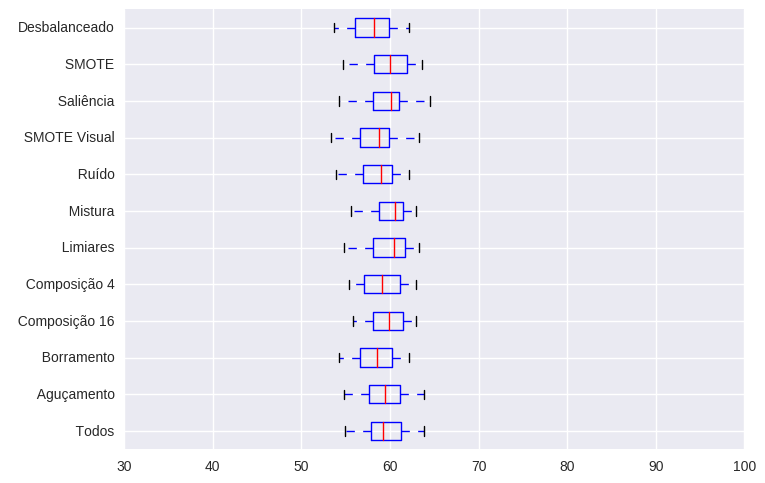
\includegraphics[width=\linewidth]{\detokenize{figuras/resultados/3/LBP_Luma_corel.png}}
  \end{center}
  \caption[Experimento com as 10 classes da base Corel. Foi utilizado o método Luma para conversão em escala de cinza e LBP como método de extração de características.]{Experimento com as 10 classes da base Corel. Foi utilizado o método Luma para conversão em escala de cinza e LBP como método de extração de características. \textit{Fonte:~Elaborado pela autora.}}
  \label{fig:resultados:3:melhor}
\end{figure}
\end{minipage}

\begin{table}[!htbp]
\centering
\caption{Experimento com as 10 classes da base Corel.}
\label{my-label}
\begin{tabular}{|l|c|c|}
\hline
\textbf{Luma e LBP} & \textbf{Média} & \textbf{Desvio padrão} \\ \hline
Todos               & 59.46          & 2.23                   \\ \hline
Aguçamento          & 59.32          & 2.33                   \\ \hline
Borramento          & 58.41          & 2.36                   \\ \hline
Composição 16       & 59.71          & 1.92                   \\ \hline
Composição 4        & 58.97          & 2.20                   \\ \hline
Limiares            & 59.89          & 2.33                   \\ \hline
Mistura             & \textbf{59.99} & 2.02                   \\ \hline
Ruído               & 58.48          & 2.21                   \\ \hline
SMOTE Visual        & 58.43          & 2.35                   \\ \hline
Saliência           & 59.63          & 2.07                   \\ \hline
SMOTE               & 59.78          & 2.36                   \\ \hline
Desbalanceado       & 58.09          & 2.31                   \\ \hline
\end{tabular}
\end{table}

%-------------------------------------------------------------------------------
\item[] \textbf{Resultado da maior variância obtida com a combinação dos métodos de extração e conversão para escala de cinza}

\begin{minipage}{\linewidth}
  \begin{figure}[H]
    \begin{center}
        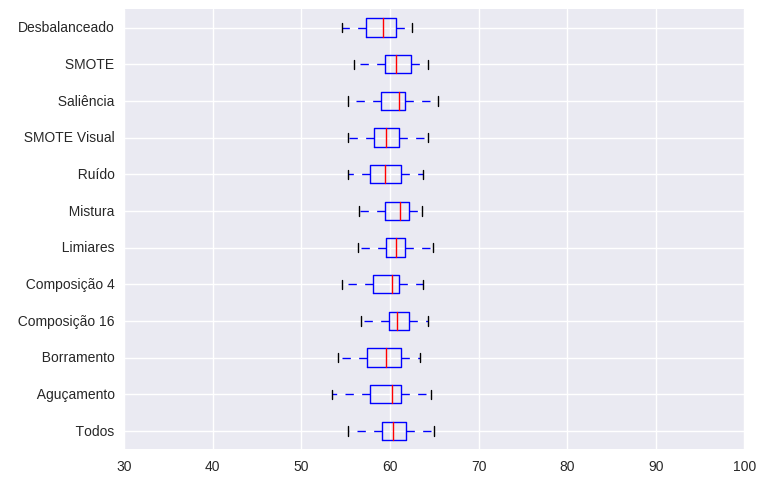
\includegraphics[width=\linewidth]{\detokenize{figuras/resultados/3/LBP_Intensity_corel.png}}
    \end{center}
    \caption[Experimento com as 10 classes da base Corel. Foi utilizado o método \emph{Intensidade} para conversão em escala de cinza e LBP como método de extração de características.]{Experimento com as 10 classes da base Corel. Foi utilizado o método \emph{Intensidade} para conversão em escala de cinza e LBP como método de extração de características. \textit{Fonte:~Elaborado pela autora.}}
    \label{fig:resultados:3:pior}
  \end{figure}
\end{minipage}

\begin{table}[]
\centering
\caption{My caption}
\label{my-label}
\begin{tabular}{|l|c|c|}
\hline
\textbf{LBP Intensity} & \textbf{Média}     & \textbf{Desvio Padrão} \\ \hline
Todos                  & 60.39          & 2.35               \\ \hline
Aguçamento             & 59.78          & 2.51               \\ \hline
Borramento             & 59.30          & 2.34               \\ \hline
Composição 16          & \textbf{60.73} & 2.23               \\ \hline
Composição 4           & 59.77          & 2.30               \\ \hline
Limiares               & 60.59          & 2.24               \\ \hline
Mistura                & 60.71          & 2.16               \\ \hline
Ruído                  & 59.39          & 2.44               \\ \hline
SMOTE Visual           & 59.44          & 2.26               \\ \hline
Saliência              & 60.36          & 2.18               \\ \hline
SMOTE                  & 60.49          & 2.22               \\ \hline
Desbalanceado          & 58.91          & 2.20               \\ \hline
\end{tabular}
\end{table}

%-------------------------------------------------------------------------------
\item[] \textbf{Discussão}

\end{itemize}

%%%%%%%%%%%%%%%%%%%%%%%%%%%%%%%%%%%%%%%%%%%%%%%%%%%%%%%%%%%%%%%%%%%%%%%%%%%%%%%%
\FloatBarrier
\subsection{Experimento 4: classes naturalmente desbalanceadas}

\begin{itemize}
%-------------------------------------------------------------------------------
\item[] \textbf{Base de Imagens}


%-------------------------------------------------------------------------------
\item[] \textbf{Protocolo}

O seguinte protocolo foi seguido para a obtenção dos resultados:

\begin{enumerate}
\item \textbf{Classes de imagens originais}:
\item \textbf{Desbalanceamento}:
\item \textbf{Método para geração artificial}:
\item \textbf{Quantização}:
\item \textbf{Extração de características}:
\item \textbf{Classificação}:
\end{enumerate}
%-------------------------------------------------------------------------------
\item[] \textbf{Resultados e Discussão}

\end{itemize}

%%%%%%%%%%%%%%%%%%%%%%%%%%%%%%%%%%%%%%%%%%%%%%%%%%%%%%%%%%%%%%%%%%%%%%%%%%%%%%%%
\FloatBarrier
\subsection{Experimento 5: classes com muitas imagens}

\begin{itemize}
%-------------------------------------------------------------------------------
\item[] \textbf{Base de Imagens}


%-------------------------------------------------------------------------------
\item[] \textbf{Protocolo}

O seguinte protocolo foi seguido para a obtenção dos resultados:

\begin{enumerate}
\item \textbf{Classes de imagens originais}:
\item \textbf{Desbalanceamento}:
\item \textbf{Método para geração artificial}:
\item \textbf{Quantização}:
\item \textbf{Extração de características}:
\item \textbf{Classificação}:
\end{enumerate}
%-------------------------------------------------------------------------------
%-------------------------------------------------------------------------------
\item[] \textbf{Resultado da melhor combinação dos métodos de extração e conversão para escala de cinza}

\begin{minipage}{\linewidth}
  \begin{figure}[H]
  \begin{center}
      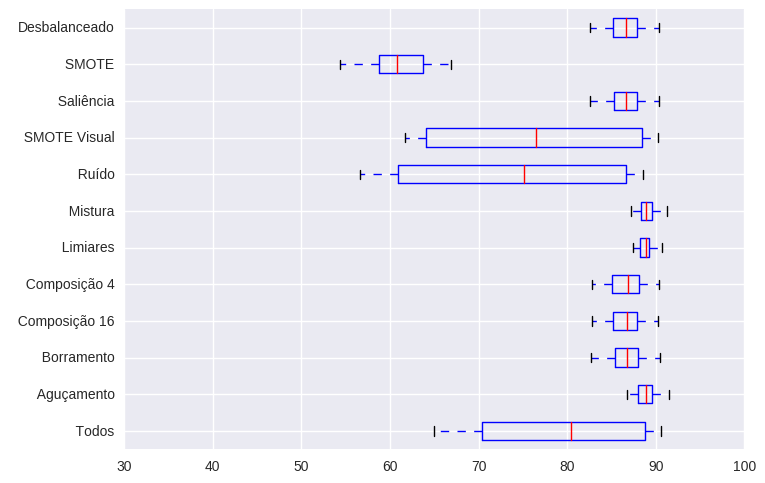
\includegraphics[width=\linewidth]{\detokenize{figuras/resultados/5/HOG_Gleam_deer-ship.png}}
  \end{center}
  \caption[]{\textit{Fonte:~Elaborado pela autora.}}
  \label{fig:resultados:5:melhor}
\end{figure}
\end{minipage}

\begin{table}[!htbp]
\centering
\caption{Experimento com 2 classes contendo 5000 imagens cada.}
\label{my-label}
\begin{tabular}{|l|c|c|}
\hline
\textbf{Gleam e HOG} & \textbf{Média} & \textbf{Desvio padrão} \\ \hline
Todos                & 79.38          & 9.88                   \\ \hline
Aguçamento           & 88.88          & 1.13                   \\ \hline
Borramento           & 86.69          & 1.81                   \\ \hline
Composição 16        & 86.61          & 1.84                   \\ \hline
Composição 4         & 86.69          & 1.97                   \\ \hline
Limiares             & 88.93          & 1.04                   \\ \hline
Mistura              & \textbf{88.99} & 0.98                   \\ \hline
Ruído                & 73.72          & 13.18                  \\ \hline
SMOTE Visual         & 76.23          & 12.51                  \\ \hline
Saliência            & 86.61          & 1.86                   \\ \hline
SMOTE                & 60.90          & 3.46                   \\ \hline
Desbalanceado        & 86.60          & 1.86                   \\ \hline
\end{tabular}
\end{table}

\end{itemize}

%%%%%%%%%%%%%%%%%%%%%%%%%%%%%%%%%%%%%%%%%%%%%%%%%%%%%%%%%%%%%%%%%%%%%%%%%%%%%%%%
% \begin{figure}[!htbp]
%   \begin{center}
%     \begin{subfigure}{.49\linewidth}
%       \centering
%       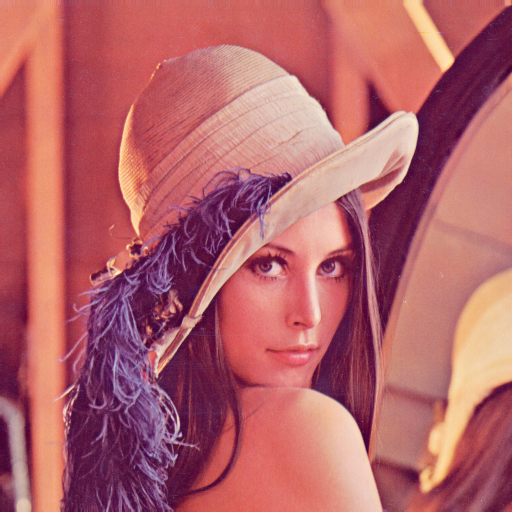
\includegraphics[width=\linewidth]{\detokenize{figuras/visualizacao/original.png}}
%     \end{subfigure}
%     \begin{subfigure}{.49\linewidth}
%       \centering
%       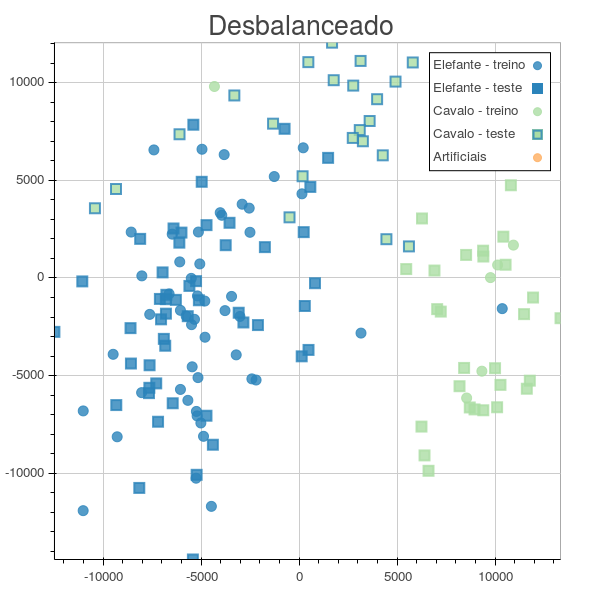
\includegraphics[width=\linewidth]{\detokenize{figuras/visualizacao/desbalanceado-fixed.png}}
%     \end{subfigure}
%   \end{center}
%   \caption{Remoção de 50\% das imagens de treino da classe Cavalo.}
%   \label{fig:desbalanceado}
% \end{figure}

%-------------------------------------------------------------------------------

%  Os resultados foram obtidos utilizando a base de imagens COREL-1000\footnote{Disponível em http://wang.ist.psu.edu/docs/related/}, composta por fotografias que representam classes variadas: tribos africanas, praia, construções, ônibus, dinossauros, elefantes, flores, cavalos, montanhas e tipos de comidas. São 10 classes balanceadas com 100 imagens cada. Para fins de exemplificação, são apresentadas amostras das imagens que representam essas classes na Figura \ref{fig:corel}.
%
%  \begin{figure}[hbpt]
%  \begin{center}
%    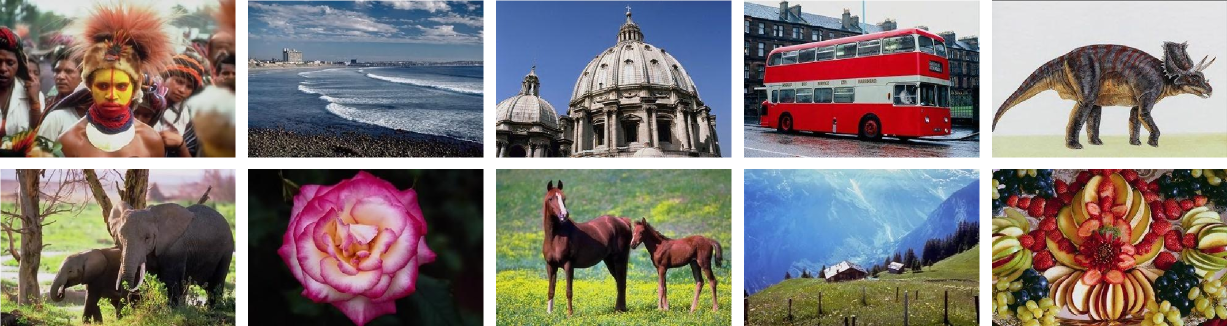
\includegraphics[width=1\linewidth]{\detokenize {figuras/exemplos_corel.png}}
%  \end{center}
%   \caption[Base de imagens COREL-1000.]{Base de imagens COREL-1000 utilizada. Estão representadas as 10 classes da base. \textit{Fonte: Elaborado pela autora.}}
%  \label{fig:corel}
% \end{figure}

% Inicialmente o classificador Naive Bayes foi explorado, apresentando melhora na acurácia ao apenas replicar as imagens. Esse comportamento não é desejado em um classificador para a avaliação de rebalanceamento de classes. O código desenvolvido para esses resultados preliminares está disponível em \url{https://bitbucket.org/moacirponti/imagefeatureextraction/overview}.

% As etapas para a geração das imagens artificiais, passo \ref{item} da seção anterior, foram:
%
% \begin{enumerate}
% \item Selecionar uma imagem aleatoriamente do conjunto de treino;
% \item Selecionar uma operação aleatória entre: borramento, adição de ruído, \textit{unsharp mask}, mistura ou composição;
% \begin{enumerate}
% \item Caso seja selecionada a composição: encontrar uma outra imagem aleatória, selecionar um quadrante dessa imagem e novamente uma operação entre: borramento, adição de ruído, \textit{unsharp mask} ou mistura;
% \end{enumerate}
% \item Aplicar essa operação na imagem previamente selecionada e adicionar essa imagem gerada ao conjunto de treino;
% \item Repetir os passos 2 a 4 até que as classes estejam igualmente balanceadas.
% \end{enumerate}

% Este estudo apresentou evidências experimentais de que, em problemas de duas classes (apresentadas na Figura~\ref{fig:praiamontanha}), pode haver ganho estatístico da medida-F ao gerar imagens, quando comparado à geração de exemplos artificiais no espaço de atributos (ou seja, depois que as características já foram extraídas das imagens). Essa melhoria pode ser notada na Figura~\ref{fig:resultmelhor}, que apresenta a relação da medida-F com a taxa de balanceamento, utilizando: as imagens originais, a geração de exemplos com SMOTE e as imagens geradas. Para essa configuração, foi utilizado o descritor de características ACC com a conversão em escala de cinza por MSB e a operação de pré-processamento por combinação. As classes ``praia'' e ``montanha'' foram escolhidas por serem as classes que possuem maior dificuldade de diferenciação, havendo alta taxa de sobreposição de intensidades de cores e texturas, conforme testes realizados.

% Também foi possível notar que algumas operações não provocaram a melhora da classificação. A operação de adição de ruído para geração artificial, a posterior extração utilizando CCV e a quantização por MSB, destacou-se como o pior resultado, apresentado na Figura~\ref{fig:resultpior}. Outros casos que não obtiveram o resultado esperado envolveram as operações de borramento e de \textit{unsharp masking}.

% Após a realização dos testes, as operações que melhor se destacaram foram: utilizar todas as operações, apenas mistura e apenas composição. E as operações que resultaram em uma classificação pior do que o uso do SMOTE foram: utilizar apenas borramento, ruído ou \textit{unsharp masking}. Com o teste estatístico de Friedman foi possível verificar que o ACC foi o extrator que melhor se beneficiou das características geradas; e CCV e GCH os menos beneficiados. \enlargethispage{-\baselineskip} A Tabela \ref{tab:result} apresenta os \textit{rankings} encontrados por este teste para todas as execuções das melhores operações. O p-valor computado corresponde a $4.24E^{-11}$, assim a hipótese nula de que não há diferença entre as execuções foi rejeitada. Vale destacar que para algumas execuções, o teste de Friedman retornou o \textit{ranking}: geração artificial (1), SMOTE (2) e imagens originais (3), ou seja, sem que SMOTE e a geração artificial concorressem pela mesma posição, diferente da tabela apresentada.
%
% \begin{table}[htb]
% \centering
% \caption{Posição média dos algoritmos utilizando Friedman}
%   \begin{tabular}{c|c}
%     Algoritmos  &   Posição \\ \hline
%     Original    &   3.0000  \\
%     Smote       &   1.6136  \\
%     Artificial  &   1.3863  \\
%   \end{tabular}
%  \label{tab:result}
% \end{table}
%
% Em outro experimento, utilizou-se as cópias das imagens de treino para rebalancear, sem realizar nenhuma operação de pré-processamento (método conhecido como SRS - \textit{Simple Random Sampling}). A Figura~\ref{fig:resultcopia} mostra as respectivas medidas-F encontradas. É possível notar que a cópia dessas imagens não adiciona nenhuma informação nova para o aprendizado.
%
% \begin{figure}[htb]
%  \begin{center}
%    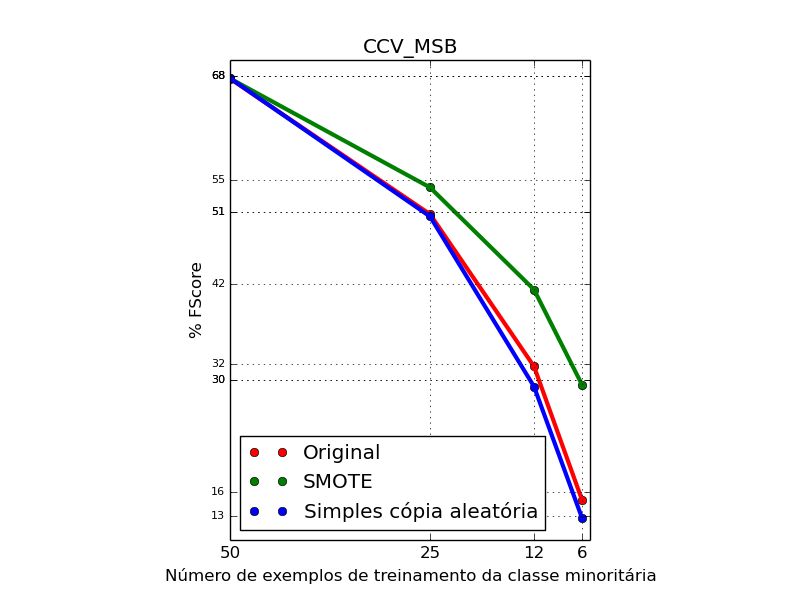
\includegraphics[width=\linewidth]{\detokenize {figuras/resultado-copia.png}}
%  \end{center}
%   \caption[Simples replicação de exemplos sem realizar nenhuma operação.]{Simples replicação de exemplos sem realizar nenhuma operação de pré-processamento. É possível verificar que não foi adicionada nenhuma informação relevante para o aprendizado. \textit{Fonte:~Elaborado pela autora.}}
%  \label{fig:resultcopia}
% \end{figure}
%
%
\section{Considerações Finais}

% Com os experimentos realizados foi possível notar que a geração de imagens artificiais pode gerar novas informações para a classificação das imagens. O que indica que um estudo mais aprofundado de quais operações podem ser aplicadas nas imagens originais auxilie o cenário de bases desbalanceadas.
%
% Dessa forma, esse capítulo também apresentou as próximas tarefas a serem realizadas. Foi destacada a análise das redes de convolução para identificar quais características latentes são automaticamente extraídas. Apesar de algumas operações de pré-processamento terem gerado imagens que melhoraram a classificação, algumas não causaram melhora. Isso indica que a análise da relevância da informação contida em imagens deve melhorar esse resultado. A memória associativa, aprendida com uma máquina de Boltzmann restrita, deve ser capaz de indicar se uma determinada imagem é relevante para o aprendizado.
